\documentclass[a4paper]{iacas}

\usepackage{cite}
\usepackage{hyperref}% embedding hyperlinks [must be loaded after dropping]
\usepackage{amsmath,amsthm,amssymb,amsfonts,latexsym,mathrsfs,wasysym}
\usepackage{marvosym}
\usepackage{subcaption}
\usepackage{soul,color}
\usepackage{threeparttable}% tables with footnotes
\usepackage{dcolumn}% decimal-aligned tabular math columns
\usepackage{float}
\usepackage{graphicx}
\usepackage{accents}
\usepackage{tikz}
\usepackage{lastpage}
\usepackage{fancyhdr}
\usepackage{color}
\usepackage{cancel}
\usepackage{setspace}
%\doublespacing
% or:
\onehalfspacing
%\usepackage[T1]{fontenc}
%\usepackage{bigfoot} % to allow verbatim in footnote
\usepackage[framed,numbered]{matlab-prettifier}
\pagestyle{plain}
%\usepackage[hebrew,english]{babel}
\usetikzlibrary{shapes.geometric, arrows, calc}

\newcolumntype{d}{D{.}{.}{-1}}
\graphicspath{{figures/}}

% define some commands to maintain consistency
\newcommand{\pkg}[1]{\texttt{#1}}
\newcommand{\cls}[1]{\textsf{#1}}
\newcommand{\file}[1]{\texttt{#1}}
\newcommand{\sgn}[1]{\operatorname{sgn}\left(#1\right)}
\newcommand{\sat}[1]{\operatorname{sat}\left(#1\right)}
\newcommand{\rrule}[1]{\rule[#1]{0pt}{0pt}}
\newcommand{\fracds}[2]{\frac{\displaystyle #1\rrule{-0.2em}}{\displaystyle #2\rrule{1em}}}
\newcommand{\figref}[1]{Fig.~\ref{#1}}
\newcommand{\ubar}[1]{\underaccent{\bar}{#1}}
\newcommand{\norm}[1]{\lvert \lvert \vec #1 \rvert \rvert}

%diffeomorphism

\begin{document}

\begin{center}
 \large Introduction to Machine Learning - 236756
 \end{center}
\begin{center}
\large\textbf{Homework \#2}
 \end{center}


\begin{tabular}{l}
\\
{\bf\textit{Alexander Shender 328626114}} \\
{\bf\textit{Snir Hordan XXXXXXXXX}} \\
Technion - Israel Institute of Technology
\end{tabular}

\vspace{2em}

\section{Part 2 - Dry Assignment}

\subsection{Part 2a}
The halfspace is homogeneous if the hyperpalce which defines them passed through the origin.
Subsequently, the non-homogeneous halfspaces have to be defined by a hyperplance which is displaced by some parameter
$b$ (bias) from the origin.

We include this bias $b$ term in the parameters $w$, thus bringing $w$ to $R^(d+1)$, which is denoted $z \in R^(d+1)$ in the assignment.
But this term doesn't have to be multiplied by any input, thus we simply add '1' to the input vector $x$. The answer is thus:

$$ g : R^d \rightarrow R^{d+1} = (x, 1) $$
$$ z : R^d \rightarrow R^{d+1} = (w, b) $$


\newpage
\subsection{Part 2b}



First, some general notes on Datasets:
\begin{itemize}
  \item the datasets A and C are not linearly separable in the original dimension
  \item the dataset B is linearly separable in original dimension
\end{itemize}


Some general notes on models:
\begin{itemize}
  \item Perceptron can only classify linearly separable cases
  \item KNN can classify non-linear datasets, non-parametric
  \item Decision trees can classify non-linear datasets as well
\end{itemize}


YES = can fit
NO = cannot fit


\begin{enumerate}
  \item Perceptron

\begin{itemize}
  \item A: NO. The dataset is not linearly separable. This is actually similar to the XOR function, which cannot be learned by any linear model.
  \item B:YES. The dataset is easily linearly separable.
  \item C: NO. The dataset is not linearly separable. Only using the Kernel Trick (e.g. polynomial of 2nd order) can bring the dataset to a higher dimension, where they can be separated by a hyperplane.
\end{itemize}

  \item KNN, $k=1$

\begin{itemize}
  \item A: NO. As a simple example, it can be seen that on the far left on the border between the two groups there exists an orange dot really close to the blue ones. Using KNN with $k=1$ it would classify this point as belonging to the blue group.

\begin{figure}[h!]
  \centering
  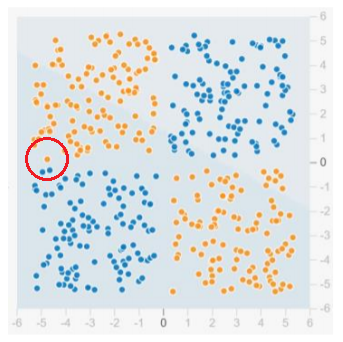
\includegraphics[width=0.4\linewidth]{q2_1.png}
  \caption{wrongly classified point at k=1}
  \label{fig:q2_1}
\end{figure}

  \item B: NO. The following point (orange) will be classified wrong, since its closest point is blue.
\begin{figure}[h!]
  \centering
  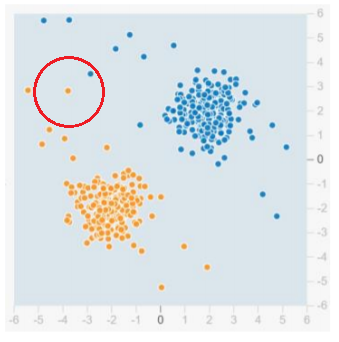
\includegraphics[width=0.4\linewidth]{q2_2.png}
  \caption{wrongly classified point at k=1}
  \label{fig:q2_2}
\end{figure}
  \item C: YES. From visual observation, all points would be classified correctly.
\end{itemize}

  \item KNN, $k=3$

\begin{itemize}
  \item A: NO. Same point as in the case with $k=1$, this point would have a majority of 2 blue points in it's proximity, resulting in a wrong classification.
  \item B: YES. From visual observation.
  \item C: YES. From visual observation.
\end{itemize}

  \item Decision tree

\begin{itemize}
  \item A: YES. The decision tree can classify non-linear datasets, and in this example, it would require exactly 4 leaves to classify all the training dataset. It may look like this:
\begin{figure}[h!]
  \centering
  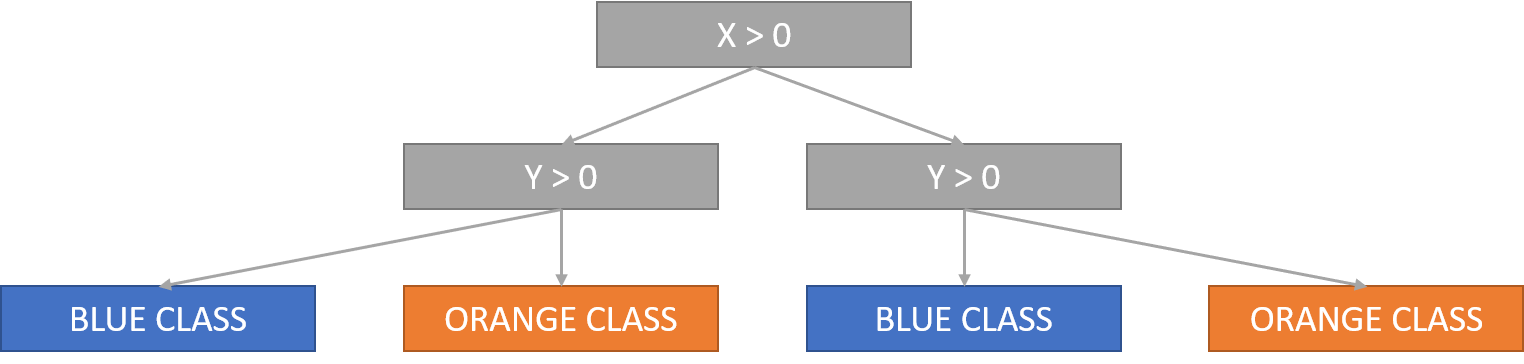
\includegraphics[width=\linewidth]{q2_3.png}
  \caption{Decision tree for Dataset A with 4 leaves}
  \label{fig:q2_3}
\end{figure}
  \item B: By having the limitation of 4 leaves, this dataset cannot be classified with 0 training error.
  \item C: Same as with B. By having limitless Decision tree depth this would be possible
\end{itemize}

\end{enumerate}


\newpage
\subsection{Part 3.1}

To find the derivative with respect to the model parameters $w_{j}, j = 1... d$, we first write the cost function explicitly for both cases
of the classification, since the cost function is defined diferently for the case where $y = 0$ and $y = 1$.


First, we denote shortly the sigmoid function with parameters $w$:
$$\sigma_{w}(x) = \frac{1}{1 - e^{-w^Tx}}$$

Thus, we can rewrite the cost function:

$$C = cost(x_{i}, y_{i}, w) = y_{i} \cdot log(\sigma(x_{i}, w)) + (1-y_{i} )\cdot log(1-\sigma(x_{i}, w))$$

This way, the left side is active for the case with $y = 1$, and the right side for the case where $y = 0$. We also take $y_{i}$ out of the sigmoid function.
It's worth noticing that the function is always negative except of the point where it is equal zero, when all predictions are perfectly correct. Thus,
this is called the gradient ascend, since we are trying to "climb" to increase the "cost" function. Here the term "cost" has the opposite measning, i would better denote it
"reward", since we are trying to maximize it.

Now we can calculate the derivatives with regards to the model parameters $w$. We summarize over all of the samples in a set.

Remembering:
$$\frac{\delta}{\delta w} log(f(w)) = \frac{1}{f(w)}(\frac{\delta}{\delta w} f(w)) $$

$$\frac{\delta C}{\delta w_j} = \frac{1}{m}  \cdot \sum_{i=1}^{m}  ((y_{i}) \cdot \frac{1}{\sigma(x_{i},w)} \cdot \frac{\delta \sigma(x_{i},w)}{\delta w_{x_{i}}}) + \\ 
((1-y_{i}) \cdot \frac{1}{(1-\sigma(x_{i},w))} \cdot \frac{\delta (1-\sigma(x_{i},w))}{\delta w_{x_{i}}})$$

We calculate the partial derivatives of the sigmoid function with respect to the model parameters using the chain rule and the hint in the assignment.

$$\frac{\delta \sigma(x_{i},w)}{\delta w_{x_{i}}}  = \frac{\delta \sigma(x_{i},w)}{\delta (x_{i},w)} \cdot \frac {\delta (x_{i},w)}{\delta (w)} =  \sigma(x_{i},w) \cdot (1-  \sigma(x_{i},w)) \cdot x_{i_{j}}$$

where $x_{i_{j}}$ is the j'th parameter of the sample $x_{i}$

inserting back into the equation:

$$\frac{\delta C}{\delta w_j} = \frac{1}{m}  \cdot \sum_{i=1}^{m}  ((y_{i}) \cdot \frac{\sigma(x_{i},w) \cdot (1-  \sigma(x_{i},w))}{\sigma(x_{i},w)}   \cdot x_{i_{j}} - \\ 
((1-y_{i}) \cdot \frac{\sigma(x_{i},w) \cdot (1-  \sigma(x_{i},w))}{(1-\sigma(x_{i},w))} \cdot x_{i_{j}})$$

Shortening:

$$\frac{\delta C}{\delta w_j} = \frac{1}{m}  \cdot \sum_{i=1}^{m}  (y_{i} \cdot (1-  \sigma(x_{i},w))   \cdot x_{i_{j}} - 
((1-y_{i}) \cdot \sigma(x_{i},w) \cdot x_{i_{j}})$$
 
$$= -\frac{1}{m}  \cdot \sum_{i=1}^{m}  (y_{i} x_{i_{j}} - y_{i}x_{i_{j}} \sigma(x_{i},w) - \sigma(x_{i},w) x_{i_{j}} +  y_{i}x_{i_{j}} \sigma(x_{i},w) = \\$$

$$= -\frac{1}{m}  \cdot \sum_{i=1}^{m}  (y_{i} x_{i_{j}}  - \sigma(x_{i},w) x_{i_{j}} )$$ 

$$\frac{\delta C}{\delta w_j} = \frac{1}{m}  \cdot \sum_{i=1}^{m}  (x_{i_{j}} \cdot ( y_{i}  - \sigma(x_{i},w) )$$


We are used to the matrix form. Converting the expression to matrix form:

$$\frac{\delta C}{\delta w} = \frac {1}{m} X \cdot ( y - \sigma(X, w))$$

where $m$ is the number of samples in a set. 

\subsection{Part 3.2}

Since this is the gradient ascent algorithm, we do want to go in the direction of the steepest ascent, which is exactly the gradient. So, we update our parameters in the following way:

$$w^{t+1} = w^{t} + \eta \cdot \frac{1}{m}  \cdot \sum_{i=1}^{m}  (x_{i_{j}} \cdot ( y_{i}  - \sigma(x_{i},w^{t}) )$$

or in a matrix form:

$$w^{t+1} = w^{t} + \eta \cdot \frac {1}{m} X \cdot ( y - \sigma(X, w^{t}))$$

where :

\begin{itemize}
  \item $w^{t+1}$ - the parameters at the next iteration
  \item $w^{t}$ - the parameters are the current iteration
  \item $\eta$ - learning rate
\end{itemize}


\end{document}




